\documentclass[a4paper, 10pt, fleqn]{article}
\usepackage{../custom}
\usepackage{../pageformatting}

\usepackage[ngerman]{babel}
%mathe packages
\usepackage{amsmath}
\usepackage{booktabs}
\newcommand{\tabitem}{~~\llap{\textbullet}~~}

\graphicspath{{pdf/}{../images/}}

%============PAGE PROPERTIES=============
\newcommand{\revisiondate}{\today}
\newcommand{\documenttitle}{Clock Pendelum Analyzer} % used for title in title and subtitle pages
\newcommand{\authors}{Tobias Kreienbühl \& Daniel Föhn} %used for title page only
\newcommand{\subauthors}{im Auftrag der Hochschule Luzern} %used for title page only
\newcommand{\subtitle}{PMP}%usedfortitleandsubtitlepages
\newcommand{\documentdesc}{Ein Projekt Management Plan für \documenttitle}


\begin{document}
	\begin{titlepage}
		\titleGM
		\thispagestyle{empty}
	\end{titlepage}
	
	\tableofcontents
	\listoffigures
	\listoftables
	
	\clearpage
	\section{Einführung}
		\subsection{Zweck des Dokuments}
		\subsection{Zielpublikum}
		\subsection{Versionierung}
			\begin{table}[h]
				\centering
				\begin{tabularx}{\textwidth}{|c|c|X|}
				\hline
				\rowcolor{shadecolor}\textbf{Version} & \textbf{Datum} & \textbf{Kommentar}\\ \hline
				V1.0 & 28.09.2017 & initiale datei \\ \hline
                V1.1 & 29.09.2017 & rahmenplan und projektrisiken\\
				\end{tabularx}
			\end{table}
		\subsection{Glossar}
			\begin{description}
				\item[Abkürzung]- Erklärung
			\end{description}

\subtitlepage{Projektmanagement}
	\section{Projektorganisation}
        \begin{figure}[H]
            \centering
            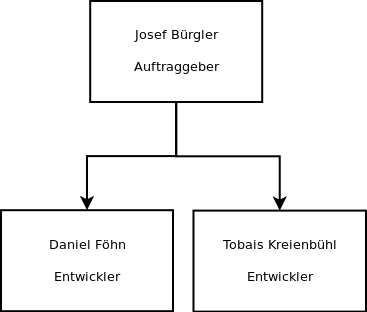
\includegraphics[width=.5\textwidth]{organisation.png}
            \caption{einfache Projektorganisationsstruktur}
        \end{figure}
		\textbf{Entwickler:} Tobias Kreienbühl
        \begin{itemize}
            \item Projektplanung
            \item Entwicklung der Software
            \item Entwicklung der Mechanik
            \item Mathematische Umsetzung
        \end{itemize}
        \vspace{.5cm}
        \textbf{Entwickler:} Daniel Föhn
        \begin{itemize}
            \item Projektplanung
            \item Entwicklung der Software
            \item Entwicklung der Elektronik
            \item Aufbau der Environment
        \end{itemize}
        \vspace{.5cm}
        \textbf{Auftraggeber:} Josef Bürgler
        \begin{itemize}
            \item Anforderungen abnehmen
            \item 
        \end{itemize}
    
    \clearpage
	\section{Projektrahmenplan}
        In diesem Kapitel werden die Meilensteine und Eckdaten wie Start- und Endzeitpunkt des Projekts festgehalten.
        \begin{figure}[H]
            \centering
            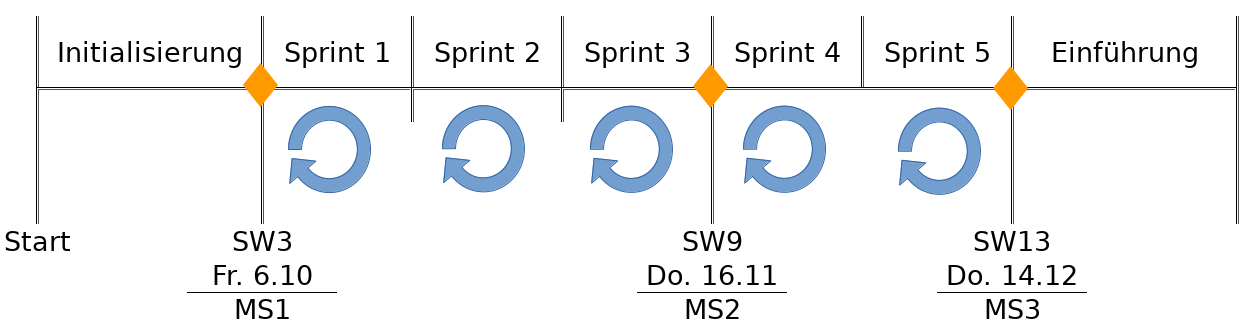
\includegraphics[width=\textwidth]{../../rahmenplan.png}
            \caption{Rahmenplan mit Phasen, Meilensteine und Sprints}
        \end{figure}
        \begin{tabularx}{\textwidth}{lll}
            \textbf{MS1} & Zeitpunkt: & Freitag 6.10.\\
            & Artefakte: & \tabitem PMP\\
            & & \tabitem Entwurf des Grobkonzepts\\
            & Ergebnisse: & \tabitem definierte Vorgehensart\\
            & & \tabitem Rahmenplanung\\
            & & \tabitem Vision (Scope, Ziele etc) im Grobkonzept\\
            \textbf{MS2} & Zeitpunkt: & Donnerstag 16.11.2017\\
            & Artefakte & \tabitem Prototyp 1\\
            & Ergebnisse: & \tabitem lauffähiger 1. Prototyp\\
            & & \tabitem 80\% der Sys Spec\\
            \textbf{MS3} & Zeitpunkt: & Donnerstag 14.12.2017\\
            & Artefakte & \tabitem PMP \\
            & & \tabitem SysSpec \\
            & & \tabitem Arbeitsjournal \\
            & & \tabitem Prototyp 2\\
            & Ergebnisse: & \tabitem lauffähiger 2. Prototyp\\
            & & \tabitem fertige System Spezifikation (Projektreport)\\
            & & \tabitem fertiger PMP\\
        \end{tabularx}
    \clearpage
	\section{Zeitplanung}
        Das Projekt wird mit einer agilen Zeitplanung in Form von Sprints durchgeführt. Ein Sprint dauert jeweils 2 Wochen.
        \begin{figure}[H]
            \centering
            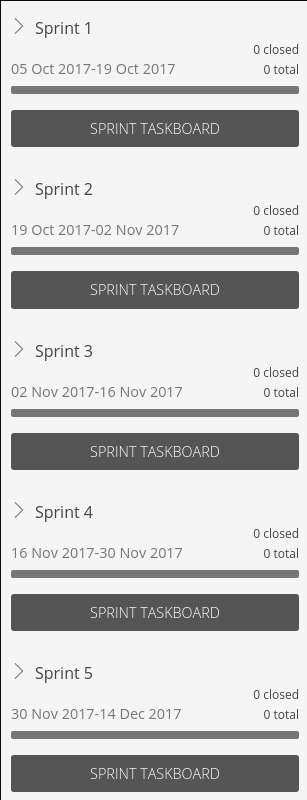
\includegraphics[width=.5\textwidth]{sprint_overview.png}
        \end{figure}

    \clearpage
    %!TEX root = Projektdokumentation_ClockPendulumAnalyzer.tex
\newcommand*{\risk}[2]{
    \begingroup
    \ifnum #1>#2
    \cellcolor{red}
    \fi
    \endgroup
}

\section{Risikomanagement}
    In diesem Kapitel werden allfällige Risiken identifiziert, bewertet und verwaltet. 
    \subsection{Risikobewertung}
    Im Projekt wurden folgende Risiken (Tabelle \ref{tab:risks}) identifiziert und anhand der Auswirkung und Eintrittswahrscheinlichkeit bewertet. Die Bewertungsmatrix in Bild \ref{fig:riskmatrix} zeigt die möglichen Risikowerte auf.
    \begin{table}[H]
        \centering
        \begin{tabular}{|l|l|c|c|c|}
            \hline
            \textbf{Nr} & \textbf{Risiko} & \textbf{Auswirkung} & \textbf{Eintrittsw'keit} & \textbf{Risikowert}\\ \hline
            1 & Fehlerhafte Implementation & 2 & 2 & \cellcolor{yellow}4\\ \hline
            2 & Teammitglied fällt aus & 2 & 2 & \cellcolor{yellow}4\\ \hline
            3 & Auftraggeber fällt aus & 1 & 1 & \cellcolor{green}1\\ \hline
            4 & Teamdifferenzen & 2 & 1 & \cellcolor{green}2\\ \hline
            5 & Verlust des Programmcodes & 3 & 1 & \cellcolor{yellow}3\\ \hline
            6 & Motivation verschwindet & 2 & 1 & \cellcolor{green}2\\ \hline
            7 & Fehlende Kommunikation mit Stakeholder & 3 & 1 & \cellcolor{yellow}3\\ \hline
            8 & RTC Module kommen zu spät & 3 & 1 & \cellcolor{yellow}3\\ \hline
            9 & Eingeschränkte Debugging Funktionalität & 2 & 3 & \cellcolor{red}6\\ \hline
            10 & Hardwareteile gehen kaputt & 2 & 2 & \cellcolor{yellow}4\\ \hline
            11 & Projektreport geht verloren & 3 & 1 & \cellcolor{yellow}3\\ \hline
            12 & Testuhr geht verloren & 2 & 1 & \cellcolor{green}2\\ \hline
            13 & Umsetzung entspricht nicht den Erwartungen & 3 & 2 & \cellcolor{red}6\\ \hline
        \end{tabular}
        \caption{Tabelle der identifizierten Risiken}
        \label{tab:risks}
    \end{table}
    
    \begin{figure}[H]
        \centering
        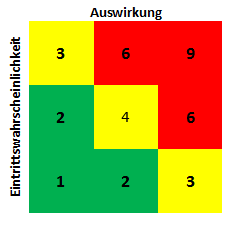
\includegraphics{Risikomatrix.png}
        \caption{Risikobewertung in einer 3x3 Matrix}
        \label{fig:riskmatrix}
    \end{figure}
    
    \clearpage
    \subsection{Massnahmenkatalog}
    Die Risiken mit einem Wert von 6 oder 9 werden als kritisch empfunden und erhalten eine Auflistung von Massnahmen gegen Auswirkung und Eintritt (Tabelle \ref{tab:arrangements}).
    \begin{table}[h]
        \centering
        \begin{tabular}{cp{7cm}p{7cm}}
            \textbf{RisikoNr} & \textbf{Massnahmen gegen Auswirkung} & \textbf{Massnahmen gegen Eintrittsw'keit}\\ \hline
            9 & \tabitem Alternative IDE für Debugging Zwecke & \tabitem Persönliche Präferenzen zurückstellen \\ \hline 
            13 & & \tabitem regelmässiges Reporting an die Stakeholder\\
            & &\tabitem gutes Requirementsengineering\\ \hline
            
        \end{tabular}
        \caption{Massnahmen gegen kritische Risiken}
        \label{tab:arrangements}
    \end{table}

    \clearpage
    %!TEX root = PMP_ClockPendelumAnalyzer.tex
\section{Test}
		\subsection{Testumgebung}
			\textit{in welcher Umgebung wurden die Tests gemacht}
		\subsection{Testfälle}
			\textit{Was wird durch das Testen abgedeckt}
			\subsubsection{Unit Tests}
			\subsubsection{Blackbox Tests}
	

\clearpage
\thispagestyle{empty}
	\section*{Anhang}
\end{document}
